\begin{Schunk}
\begin{Sinput}
> library("Ham94", lib.loc = "../../../library")
\end{Sinput}
\end{Schunk}
The above example examined the effect changing
\textgreek{f}
on the dynamic multiplier.  Pages 5 and 6 
describe what happens when the permanence of the change is varied with a fixed multiplier, i.e.
while leaving
\textgreek{f}
unchanged.
\begin{Schunk}
\begin{Sinput}
> phi <- 0.8
> T <- 20
> w <- 1 * cbind(1:T == 6, 1:T >= 6)
> y <- array(dim = c(T, 2))
> y[1:5, ] <- 0
> for (j in 6:T) y[j, ] <- phi * y[j - 1, ] + w[j, ]
\end{Sinput}
\end{Schunk}
The results can be plotted reproducing figures 1.2 and 1.3.
\begin{center}
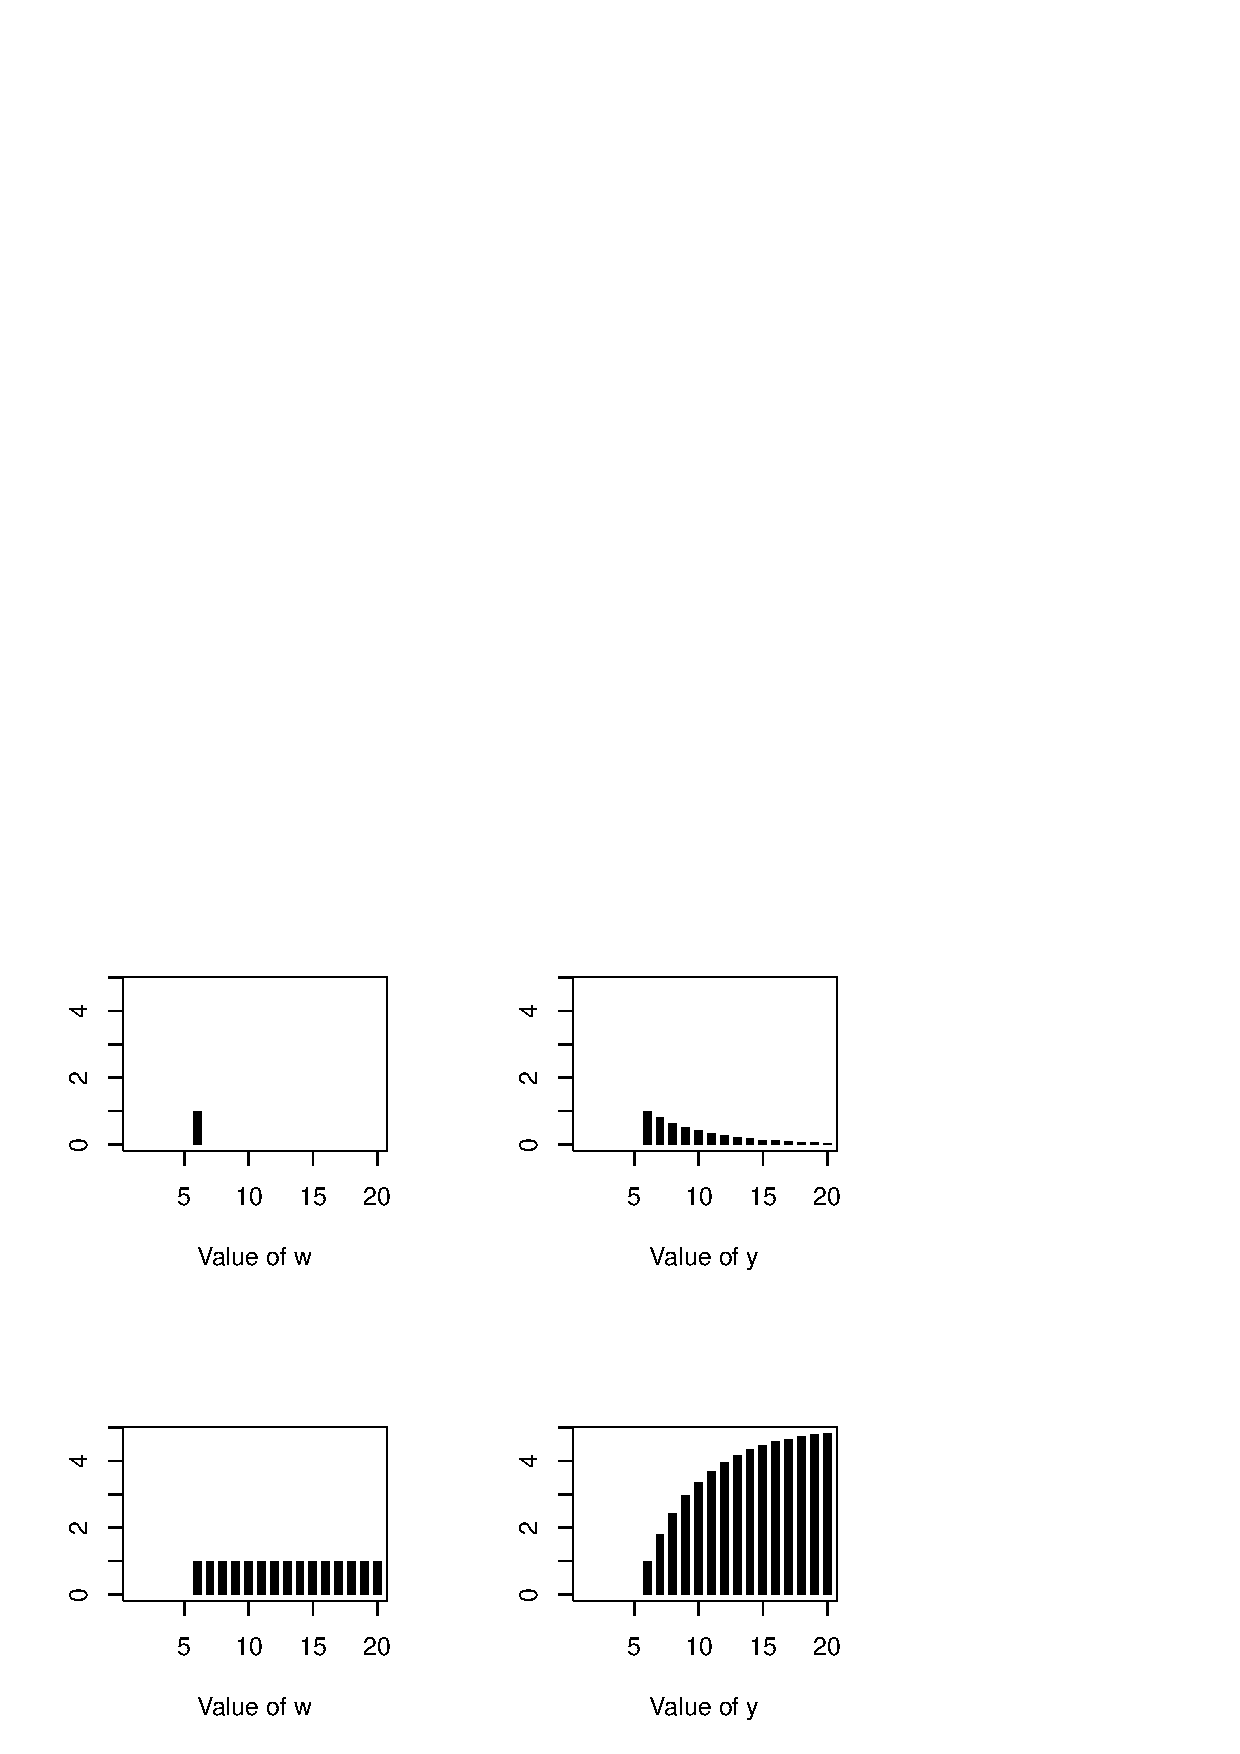
\includegraphics{p5-003}
\end{center}
